
\section{量子谐振子与厄密方程}
自然界广泛存在简谐振动,任何体系在平衡位置附近的小振动,例如分子振动、晶格振动、原子核表面振动以及辐射场等往往都可以分解成若干彼此独立的一维简谐振动。简谐振动往往还作为各种复杂运动的初步近似。研究简谐振动,无论在理论还是在应用上都是很重要的。
\subsection{谐振子的势函数}
\begin{example} %1
试求相互作用势函数V(x) 在平衡位置附近的二阶近似\\
\end{example}
\begin{proof}
半经验的Lennard-Jones势,如图所示\\
\centerline{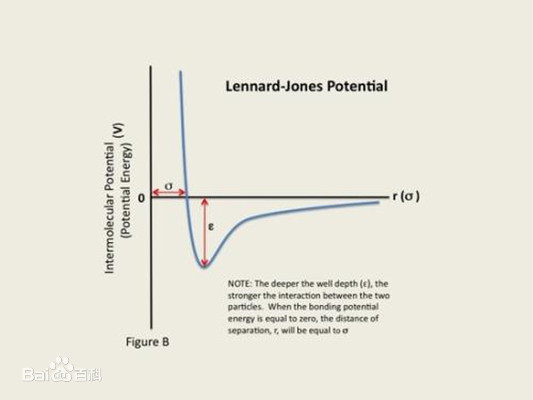
\includegraphics[width=0.5\textwidth]{LJpotential}}  
量子的势函数比L-J 势更加复杂,但不管有多复杂在平衡位置 ($x=a$)附近都可做泰勒展开
 \begin{equation*}
V(x)=V(a) +\frac{1}{1!} \frac{\partial V}{\partial x} |_{x=a} (x-a) +\frac{1}{2!} \frac{\partial ^2 V}{\partial x ^2} |_{x=a} (x-a) ^2 + ... 
\end{equation*}
很明显,一阶导应为零,因此, 二阶近似可写为 \\
$\displaystyle  \begin{array}{lllllllll}
	V(x) &\approx V(a)+\frac{1}{2!} \frac{\partial ^2 V}{\partial x ^2} |_{x=a} (x-a) ^2   \\
	        & =V_0+\frac{1}{2} k (x-a) ^2 
\end{array}$\\
取坐标原点为($a, V_0 $), 得:\\
 \begin{equation*}
	V(x)=\frac{1}{2} k x^2 
\end{equation*}
\end{proof}
\begin{remark}
弹簧力正是势函数V(x) 在平衡位置附近的二阶近似\\
 \begin{equation*}
	F=-\frac{ \partial V}{\partial x}=-kx 
\end{equation*}	
因此,势函数V(x) 可写成:\\
  \begin{equation*}
 	V(x)=\frac{1}{2} \mu \omega ^2 x^2 
 \end{equation*}
\end{remark}


\subsection{谐振子薛定谔方程}
\begin{example} %3
求解谐振势条件下的薛定谔方程\\
\end{example}
\begin{proof}
把势函数代入薛定谔方程, 得: 
\begin{equation*}
	i\hbar \frac{\partial }{\partial t} \Psi (x,t ) =[ -\frac{\hbar^2}{2\mu } \frac{d ^2}{x^2} + \frac{1}{2} \mu \omega ^2 x^2   ] \Psi (x, t ) 
\end{equation*}
令$\Psi (x,t) =\Psi(x) T(t) $ ,  代回方程, 时间和位置变量可分离变量:\\
解得时间函数: $T_(t)  = \exp(-i E t /\hbar) $ \\
固有函数满足定态薛定谔方程\\
\begin{equation*}
	\left [ -\frac{\hbar^2}{2\mu} \frac{\mathrm{d} ^2}{\mathrm{d} x^2} +\frac{1}{2}\mu \omega^2 x^2  \right ]\Psi(x)=E\Psi(x) 
\end{equation*}
整理:\\
\begin{equation*}
\frac{1}{\frac{\mu\omega}{\hbar}} \frac{\mathrm{d} ^2\Psi}{\mathrm{d} x^2} +	\left ( \frac{2E}{\omega \hbar} -\frac{\mu \omega}{\hbar} x^2 \right )\Psi=0
\end{equation*}
令:~~$ \xi =\alpha x$,做自变量伸缩变换 \\
\begin{equation*}
\frac{\mathrm{d} \Psi}{\mathrm{d} x} =\frac{\mathrm{d} \Psi}{\mathrm{d} \xi} \frac{\mathrm{d} \xi}{\mathrm{d} x}  = \alpha \frac{\mathrm{d} \Psi}{\mathrm{d} \xi}
\end{equation*}
\begin{equation*}
	\frac{\mathrm{d} \Psi ^2 }{\mathrm{d} x ^2} =\frac{\mathrm{d}}{\mathrm{d} x}  ( \alpha \frac{\mathrm{d} \Psi}{\mathrm{d} \xi} ) = \alpha ^2 \frac{\mathrm{d} ^2 \Psi}{\mathrm{d} \xi ^2} 
\end{equation*}
代回方程, 得\\
\begin{equation*}
	\left[ \frac{\hbar ^2 \alpha ^2 }{2\mu} \frac{\mathrm{d}}{\mathrm{d} \xi ^2}  + (E- \frac{\mu \omega ^2 \xi ^2}{2 \alpha ^2}  ) \right] \Psi(\xi) =0
\end{equation*}
同除二阶导数项系数, 得\\
\begin{equation*}
	\left[ \frac{\mathrm{d}}{\mathrm{d} \xi ^2}  + \frac{2\mu}{\hbar ^2 \alpha ^2 } (E- \frac{\mu \omega ^2 \xi ^2}{2 \alpha ^2}  ) \right] \Psi(\xi) =0
\end{equation*}
令 $\frac{\mu ^2 \omega ^2 }{\hbar ^2 \alpha ^ 4} =1$,得伸缩系数:\\
\begin{equation*}
	 \alpha ^2= \frac{\mu\omega}{\hbar}
\end{equation*}
再引入特征值\\
\begin{equation*}
\lambda = \frac{2E}{\omega \hbar}
\end{equation*}
得二阶常微分方程的标准形式:\\
\begin{equation*}
\left[ \frac{\mathrm{d} ^2\Psi}{\mathrm{d} \xi^2} + \left( \lambda - \xi^2 \right) \right] \Psi=0
\end{equation*}
\begin{remark}
n阶厄密方程有如下形式\\
	\begin{equation*}
	\frac{d^2 y}{d x^2} -2x \frac{d y}{d x} +2n y =0 
    \end{equation*}     
为了利用n阶厄密方程的结果,我们还得对谐振子固有值方程进一步简化。\\
\end{remark}
考虑渐近行为, 当 $ |x| \to \infty,  \xi \to \infty$,有 $ \xi ^2  \gg  \lambda $,方程可近似为 \\
\begin{equation*}
	\left(\frac{\mathrm{d} ^2\Psi}{\mathrm{d} \xi^2} - \xi^2 \right) \Psi=0
\end{equation*}
该方程并没有表达式解,但通过检验平方指数函数的导数\\
\begin{equation*}
	\frac{d^2 }{d \xi ^2} \exp(\frac{\xi ^2}{2}) =(\xi ^2 +1)  \exp(\frac{\xi ^2}{2}) 
\end{equation*}    
\begin{equation*}
	\frac{d^2 }{d \xi ^2} \exp( - \frac{\xi ^2}{2}) =(\xi ^2 -1)  \exp( - \frac{\xi ^2}{2}) 
\end{equation*}     
当 $ \xi \to \infty$, 这两导数可近似为:\\
\begin{equation*}
(\xi ^2 )  \exp( \frac{\xi ^2}{2}) ~~, ~~ (\xi ^2 )  \exp( - \frac{\xi ^2}{2}) 
\end{equation*}     
因此,极限状态解应与函数
\begin{equation*}
	C_1  \exp( \frac{\xi ^2}{2}) + C_2   \exp( - \frac{\xi ^2}{2})  
\end{equation*}     
相关联。但考虑到波函数的有界性,应删除发散项(第一项),得极限状态波函数的简洁形式
\begin{equation*}
\Psi_\infty (\xi)  \sim \exp( - \frac{\xi ^2}{2})  
\end{equation*}    
现考虑非极限状态,解函数可写成: 
\begin{equation*}
\Psi(\xi) = H(\xi) e^{-\xi^2/2 }  
\end{equation*}   
解函数的确定等价于多项式函数 H 的确定。

对上式求导:\\
\begin{equation*}
	\Psi'(\xi) = H'(\xi) e^{-\xi^2/2 } -  H(\xi) \xi e^{-\xi^2/2 } 
\end{equation*}  
\begin{equation*}
	\Psi''(\xi) = \left[  \left( \xi^2 -1 \right) H -2\xi H' +H''  \right] e^{-\xi^2/2}
\end{equation*}  
代回原方程  {\large $ \displaystyle \frac{\mathrm{d} ^2\Psi}{\mathrm{d} \xi^2} + \left( \lambda - \xi^2 \right) \Psi=0 $  }  \\ 
得到关于多项式$H(\xi)$的方程: \\  
\begin{equation*}
H'' -2 \xi H' +(\lambda -1) H=0 
\end{equation*}  
取$\lambda -1= 2n $,方程转化为n阶厄密方程
\begin{equation*}
	H'' -2 \xi H' +2n H=0 
\end{equation*}  
\end{proof}	
由
\begin{equation*}
\lambda = 2n +1 = \frac{2E}{\hbar  \omega}  
\end{equation*}  
解出能量特征值(能级)
\begin{equation*}
E_n=\left(n+\frac{1}{2}\right) \hbar \omega, ~~~  ( n=0,1,2, ...)  
\end{equation*}  
幂级数方法求解n阶厄密方程,
\begin{equation*}
	H=\sum_{k=0}^{\infty} c_k \xi ^k
\end{equation*}     
可得系数递推式:
\begin{equation*}
	c_{k+2} = \frac{ 2(k-n)}{(k+2)(k+1) } c_k, ~~  \left( k=0,1,2,3, ...  \right)
\end{equation*}   
分偶数阶和奇数阶写
\begin{equation*}
 c_{2m} = (-1) ^m \frac{2^mn(n-2)(n-4) ... (n-2m+2)  } {(2m)!} c_0
\end{equation*}   
显然有 $ c_{2m} =0~, ~~(2m>n)$
\begin{equation*}
c_{n} = (-1) ^m \frac{2^mn !! } {n!} c_0, ~~~(2m=n)
\end{equation*}   
\begin{equation*}
c_{2m+1} = (-1) ^m \frac{2^m (n-1) (n-3)(n-5)...(n-2m+1)  } {(2m+1)!} c_1
\end{equation*}   
显然有 $ c_{2m+1} =0~, ~~(2m+1>n)$
\begin{equation*}
	c_{n} = (-1) ^m \frac{2^m n!! }{n!} c_1, ~~~ (2m+1=n)
	\end{equation*}  
所有系数求解,幂级数解求得,\\
	$\displaystyle \begin{cases}
		H_1(\xi)  = [1- \frac{2n}{2!} \xi^2+ \frac{2^2n(n-2)}{4!} \xi^4 -...  ] \\
		H_2(\xi)  = [\xi- \frac{2(n-1)}{3!} \xi^3+ \frac{2^2(n-1)(n-3) }{5!}\xi^5 -...  ]
	\end{cases}$ \\
n阶厄密的解为:
	\begin{equation*}
		H(\xi) =c_0H_1(\xi)+c_1 H_2(\xi).
	\end{equation*}   
	根据波函数的有界性性质, H应取多项式 (不能为无穷级数)。当n为偶数时 , $C_1=0$ , 当n为奇数时 , $C_0=0$  。\\
	为了更好地描述,可以将多项式表示为降幂排列形式,令最高次项系数为:
	\begin{equation*}
		c_n =2^n
	\end{equation*}  
	系数递推式可写为:
	\begin{equation*}
		c_{k-2} = -\frac{k(k-1) } { 2(n-k+2)}  c_k
	\end{equation*} 
	\begin{equation*}
		c_{n-2} = -\frac{n(n-1) } { 2\times2}  c_n
	\end{equation*} 
	\begin{equation*}
		c_{n-4} = (-1)^2 \frac{n(n-1)(n-2) (n-3) } { 2\times2\times 4}  2^n
	\end{equation*} 
	\begin{equation*}
		c_{n-2m} = (-1)^m \frac{n! } { 2^m (2m) !! (n-2m)!}  2^n =(-1)^m \frac{n! } {  m ! (n-2m)!}  2^{n-2m} 
	\end{equation*} 
n阶厄密方程的解为厄米多项式:
\begin{equation*}
	H(\xi) =\sum_{m=0}^{M}  (-1)^m \frac{n! } {  m ! (n-2m)!}  2^{n-2m} \xi^{n-2m} ,  ~~~ M=[n/2]
\end{equation*}   
原方程的解为
 \begin{equation*}
 	\Psi_n(\xi) = N_n \exp(-\frac{\xi ^2}{2}) H(\xi) 
 \end{equation*}   
归一化得系数后,为
\begin{equation*}
	\Psi_n(x) = \left( \frac{\alpha}{\sqrt{\pi} 2^n n!}  \right) ^{1/2}  \exp(-\frac{ \alpha^2 x^2}{2}) H( \alpha x) 
\end{equation*}  
定态波函数为
\begin{equation*}
	\Psi_n(x,t) = \left( \frac{\alpha}{\sqrt{\pi} 2^n n!}  \right) ^{1/2}  \exp(-\frac{ \alpha^2 x^2}{2} -\frac{i}{\hbar} E_n t ) H( \alpha x) 
\end{equation*}  

\subsection{作业:}
1、计算积分\\ 
\[\begin{array}{lllllllll}
     \int_{0}^{+\infty} e^{-x^2 /2 dx}
\end{array}\]
2、  根据厄米多项式表达式,写出前五个厄米多项式表达式,并分析$H'_n (x)$ 与$H_{n-1} (x)$  之间的联系\\
3、 求解厄米方程\\ 
\[\begin{array}{lllllllll}
		\frac{d^2 H}{d x^2} -2x \frac{d y}{d x} +4n H =0 	
\end{array}\] 
4、  列出厄米方程的几种形式,说明厄米方程的特点\\